\documentclass[10pt,a4paper]{article}

% =========================================================================
% Packages
% =========================================================================
\usepackage{iftex}
\ifxetex
  \usepackage{fontspec}
  % Using Twentieth Century system font installed in Windows
  \IfFontExistsTF{Twentieth Century}{
    \setmainfont{Twentieth Century}[
      AutoFakeBold=2.2,
      AutoFakeSlant=0.2,
      BoldFont={Twentieth Century},
      ItalicFont={Twentieth Century},
      BoldItalicFont={Twentieth Century}
    ]
    \newfontfamily\titlefont{Twentieth Century}[
      AutoFakeBold=3.2
    ]
  }{
    \setmainfont{Twentieth-Century.ttf}[
      Path=File/Font/,
      AutoFakeBold=2.2,
      AutoFakeSlant=0.2,
      BoldFont=Twentieth-Century.ttf,
      ItalicFont=Twentieth-Century.ttf,
      BoldItalicFont=Twentieth-Century.ttf
    ]
    \newfontfamily\titlefont{Twentieth-Century.ttf}[
      Path=File/Font/,
      AutoFakeBold=3.2
    ]
  }
\else
  \usepackage[utf8]{inputenc}
  \usepackage[T1]{fontenc}
  \usepackage[scaled=0.92]{helvet}
  \renewcommand{\familydefault}{\sfdefault}
\fi
\usepackage{geometry}
\usepackage{graphicx}
\graphicspath{{Gambar/}}
\usepackage{amsmath,amssymb}
\usepackage{xcolor}
\definecolor{headerblue}{RGB}{0, 80, 160}
\usepackage{fancyhdr}
\usepackage{titlesec}
\usepackage{booktabs}
\usepackage{tabularx}
\usepackage{array}
\usepackage{caption}
\usepackage{subcaption}
\usepackage{algorithm}
\usepackage{algpseudocode}
\usepackage{hyperref}
\usepackage{microtype}
\usepackage{url}
\usepackage[nocompress]{cite}
\renewcommand\citepunct{], [}
\renewcommand\citedash{]--[}
\usepackage{float}
\usepackage{placeins}
\usepackage{enumitem}
\setlist[itemize]{label={--},leftmargin=1.5em,itemsep=1.5pt,topsep=2pt,parsep=0pt}

% =========================================================================
% Page Geometry & Margins (JTRIK Standard: A4 Paper, Margins: 2.5 cm all sides)
% =========================================================================
\geometry{
  a4paper,
  top=2.5cm,
  bottom=2.5cm,
  left=2.5cm,
  right=2.5cm,
  headheight=48pt,
  headsep=12pt,
  footskip=22pt
}

% Paragraph settings: Justified, single space, compact spacing for <= 10 pages
\setlength{\parindent}{0pt}
\setlength{\parskip}{3pt}
\linespread{1.0}

% Float Spacing Adjustments
\setlength{\floatsep}{6pt plus 2pt minus 2pt}
\setlength{\textfloatsep}{8pt plus 2pt minus 2pt}
\setlength{\intextsep}{6pt plus 2pt minus 2pt}

% Hyperlink configuration (Non-colored citations & links per JTRIK / Mendeley standard)
\hypersetup{
  hidelinks
}

% =========================================================================
% Header & Footer Settings
% =========================================================================
\pagestyle{fancy}
\fancyhf{}
\fancyhead[L]{\fontsize{9pt}{11pt}\selectfont JOURNAL OF APPLIED INFORMATION TECHNOLOGY AND COMPUTERS}
\fancyfoot[R]{\fontsize{9pt}{11pt}\selectfont\thepage}
\renewcommand{\headrulewidth}{0.4pt}
\renewcommand{\footrulewidth}{0pt}

% First page header
\fancypagestyle{firstpage}{
  \fancyhf{}
  \fancyhead[L]{%
    \begin{minipage}[c]{0.78\textwidth}
      {\fontsize{9.5pt}{12pt}\selectfont\textbf{JOURNAL OF APPLIED INFORMATION TECHNOLOGY AND COMPUTERS}}\\[2pt]
      {\fontsize{8.5pt}{10.5pt}\selectfont E-ISSN: 2797-1724, DOI: 10.000/jtrik.v1i1.2026}\\[1pt]
      {\fontsize{8.5pt}{10.5pt}\selectfont Vol. 1 No. 1 2026 pp. 01--10}
    \end{minipage}%
  }
  \fancyhead[R]{%
    \begin{minipage}[c]{0.20\textwidth}
      \raggedleft
      \IfFileExists{Gambar/image1.png}{
\includegraphics[height=1.05cm]{image1.png}}{}
    \end{minipage}%
  }
  \fancyfoot[R]{\fontsize{9pt}{11pt}\selectfont\thepage}
  \renewcommand{\headrulewidth}{0.8pt}
  \renewcommand{\headrule}{%
    \vspace{12pt}%
    {\color{headerblue}\hrule height \headrulewidth width \headwidth}%
    \vspace{-\headrulewidth}%
  }
  \renewcommand{\footrulewidth}{0pt}
}

% =========================================================================
% Section Headings Formatting
% Level 1: 13pt Bold
% Level 2: 11pt Bold
% Level 3: 10pt Bold
% =========================================================================
\titleformat{\section}
  {\fontsize{13pt}{16pt}\bfseries}{\thesection.}{0.5em}{}
\titlespacing*{\section}{0pt}{10pt}{3pt}

\titleformat{\subsection}
  {\fontsize{11pt}{14pt}\bfseries}{\thesubsection}{0.5em}{}
\titlespacing*{\subsection}{0pt}{7pt}{2pt}

\titleformat{\subsubsection}
  {\fontsize{10pt}{12pt}\bfseries}{\thesubsubsection}{0.5em}{}
\titlespacing*{\subsubsection}{0pt}{5pt}{2pt}

% Caption styles (9 pt / small)
\captionsetup{font={small},labelfont=bf,justification=centering}
\captionsetup[table]{position=top,skip=3pt}
\captionsetup[figure]{position=bottom,skip=4pt}

% =========================================================================
% Document Body
% =========================================================================
\begin{document}
\thispagestyle{firstpage}

% --- Article Title (18pt Bold) ---
{\titlefont\fontsize{18pt}{22pt}\bfseries\raggedright Development of an Offline-First Point of Sale Mobile Application with Daily Sales Forecasting Using Long Short-Term Memory (LSTM)\par}
\vspace{6pt}

% --- Authors (10pt Regular) ---
{\fontsize{10pt}{12pt}\selectfont Muhammad Kholis$^{1*}$, Zulfan Khairil Simbolon$^{2}$, Azhar$^{3}$\par}
\vspace{3pt}

% --- Affiliations (8.5pt) ---
{\fontsize{8.5pt}{11pt}\selectfont
$^{1,2,3}$ Department of Information and Computer Technology, Politeknik Negeri Lhokseumawe, Jl. Banda Aceh--Medan Km. 280.3 Buketrata, Lhokseumawe 24301, Indonesia\par}
\vspace{3pt}

% --- Corresponding Author (8.5pt) ---
{\fontsize{8.5pt}{11pt}\selectfont
*Corresponding Author: \href{mailto:parzivalxdd@gmail.com}{parzivalxdd@gmail.com}\par}
\vspace{3pt}

% --- Article Info (8.5pt) ---
{\fontsize{8.5pt}{11pt}\selectfont
\textbf{Article info:} Received August 15, 2026, Revised August 25, 2026, Accepted September 01, 2026\par}
\vspace{3pt}

% --- Open Access License (8pt) ---
{\fontsize{8pt}{10pt}\selectfont
This is an open access article under the \href{https://creativecommons.org/licenses/by-sa/4.0/}{CC BY-SA} license.\par
\vspace{2pt}
\IfFileExists{Gambar/image3.png}{
\includegraphics[height=0.70cm]{image3.png}}{%
  \IfFileExists{Gambar/template_eprotik_image1.png}{
\includegraphics[height=0.45cm]{template_eprotik_image1.png}}{}%
}\par}

\vspace{6pt}

% --- Abstract (13pt Heading, 9.5pt Regular Content) ---
{\fontsize{13pt}{15pt}\bfseries Abstract\par}
\vspace{3pt}

{\fontsize{9.5pt}{12pt}\selectfont
Micro, Small, and Medium Enterprises (MSMEs) frequently encounter challenges stemming from internet connectivity dependency in digital cashier systems, as well as high uncertainty in daily sales volume during inventory planning. This research designs and develops an offline-first mobile Point of Sale (POS) application integrating daily sales forecasting features powered by Long Short-Term Memory (LSTM), with an empirical case study at the EatsTEDI canteen, Vocational College, Universitas Gadjah Mada (SV UGM). The client application was engineered using Flutter and the local Isar Database, synchronized bidirectionally with cloud Supabase PostgreSQL, while the forecasting service runs via a containerized REST API (Flask/TensorFlow). Time series modeling was performed on 313 active days of real transaction records using log-return target transformation and benchmarked against an operational suitability threshold ($\text{sMAPE} < 20\%$). One-step-ahead forecasting evaluation recorded an average MAE of IDR 667,718.00, RMSE of IDR 897,563.00, and sMAPE of 38.06\%, indicating that the model did not reach practical operational acceptance due to data size constraints (212 training sequences) and high volatility in daily transaction patterns. Stability testing across 10 random weight initializations (multi-seed) produced an MAE spread between IDR 495,527.00 and IDR 1,048,967.00 (standard deviation of IDR 145,024.00) and an sMAPE range of 29.16\%--44.63\% (0 out of 10 seeds achieved the target threshold). Nevertheless, black-box functional testing across 12 core use cases, offline-to-online synchronization verification, and white-box logic path tracing across 7 critical functions achieved a 100\% PASS success rate, demonstrating the robust reliability of the offline-first POS architecture in ensuring uninterrupted cashier operations for MSMEs without perpetual internet connectivity.\par}

\vspace{4pt}
{\fontsize{9.5pt}{12pt}\selectfont\textbf{Keywords:} Point of Sale, Daily Sales Forecasting, Long Short-Term Memory, Offline-First, Isar DB, MSME.\par}
\vspace{6pt}

% =========================================================================
% Section 1: Introduction
% =========================================================================
\section{Introduction}

Micro, Small, and Medium Enterprises (MSMEs) represent a vital cornerstone of national economic growth in Indonesia. Nevertheless, the majority of MSME owners still administer their daily operations through manual bookkeeping or disjointed, non-integrated recording workflows \cite{sipayung2020}. In cashier point-of-sale operations, numerous business owners encounter severe operational bottlenecks caused by continuous dependency on internet connectivity \cite{siddik2020}. Pure cloud-based cashier applications frequently fail to function when network connectivity is disrupted, thereby halting payment processing and triggering customer queues. Therefore, an offline-first POS system architecture is urgently required, enabling cashier transactions to be executed locally with instant response times and synchronizing data automatically once network connectivity is restored \cite{flutter2026}.

Beyond cashier reliability at the checkout counter, another critical operational challenge confronting MSME managers is the unpredictability of daily sales volumes for supply chain logistics and inventory optimization \cite{hyndman2021}. The lack of accurate demand estimates exposes businesses to substantial financial loss resulting from stockouts as well as excessive inventory accumulation leading to perishable waste (\textit{overstocking}) \cite{box2015}. In this regard, time series forecasting provides a strategic computational mechanism for quantitatively projecting operational demands \cite{hyndman2006}.

Prior investigations have extensively evaluated computational intelligence models for retail sales demand forecasting across diverse operational settings. Moraes et al. engineered hybrid stacked and parallel CNN-LSTM models across 500 retail store time series spanning five years, yielding MAPE values of 14.15\% and 14.76\%, respectively \cite{moraes2024}. Mansur et al. proposed a CNN-LSTM architecture incorporating seven exogenous variables (such as weather and public holidays) across six months of retail sales data, achieving a MAPE of 4.16\% and outperforming standalone ANN (19.74\%) and single LSTM (10.39\%) models \cite{mansur2025}. Mitra et al. implemented LSTM neural networks with Keras Tuner hyperparameter optimization on commercial retail datasets, evidencing notable error reduction compared to traditional baselines \cite{mitra2024}. Yadav and Barde developed a real-time web-based sales prediction pipeline combining LSTM and XGBoost linked to POS registers \cite{yadav2025}. In Indonesian retail studies, Sembiring and Sary deployed LSTM for warehouse inventory replenishment, reporting MAPE values of 102--106\% compared to 85--88\% for Moving Average baselines \cite{sembiring2025}, while Jannah et al. compared LSTM and SARIMA on commercial water refill businesses \cite{jannah2025}. Furthermore, Verdiyanto et al. engineered an MSME beverage POS application embedded with Random Forest Regression \cite{verdiyanto2025}.

Although deep learning architectures such as LSTM are conceptually designed to capture complex non-linear temporal dependencies across sequential data \cite{hochreiter1997, goodfellow2016deep}, findings by Makridakis et al. in the M5 Competition underscored that simple statistical benchmarks often remain highly competitive against intricate neural networks when applied to short or volatile time series \cite{makridakis2022}. In micro-enterprise environments characterized by restricted historical records, time series models remain exceptionally sensitive to academic calendar breaks and weight initialization instability. Furthermore, previous studies have rarely benchmarked model robustness against rigorous operational feasibility thresholds or integrated forecasting inference directly into an offline-first mobile POS platform.

To address these empirical and architectural gaps, this study designs and implements an offline-first mobile Point of Sale system built with Flutter and Isar DB connected to Supabase PostgreSQL, integrated with a daily sales forecasting microservice powered by an LSTM neural network deployed via Flask on Hugging Face Spaces. The study conducts an in-depth empirical performance evaluation using both one-step-ahead forecasting and multi-seed stability testing against a practical operational threshold ($\text{sMAPE} < 20\%$) using 313 active days of real transaction records from the EatsTEDI SV UGM canteen. System verification was rigorously performed using black-box functional testing, offline synchronization validation, and white-box control path analysis across mission-critical software routines.

% =========================================================================
% Section 2: Methods
% =========================================================================
\section{Research Methods}

\subsection{Research Workflow}
This research was conducted under a quantitative Research and Development (R\&D) paradigm. The methodology comprises two interconnected core phases: the design and engineering of the offline-first Point of Sale application, and the development and empirical evaluation of the LSTM time series forecasting model, as depicted in Figure \ref{fig:alur_penelitian}.

\begin{figure}[htbp]
  \centering
  \IfFileExists{Gambar/arsitektur_sistem_bw.png}{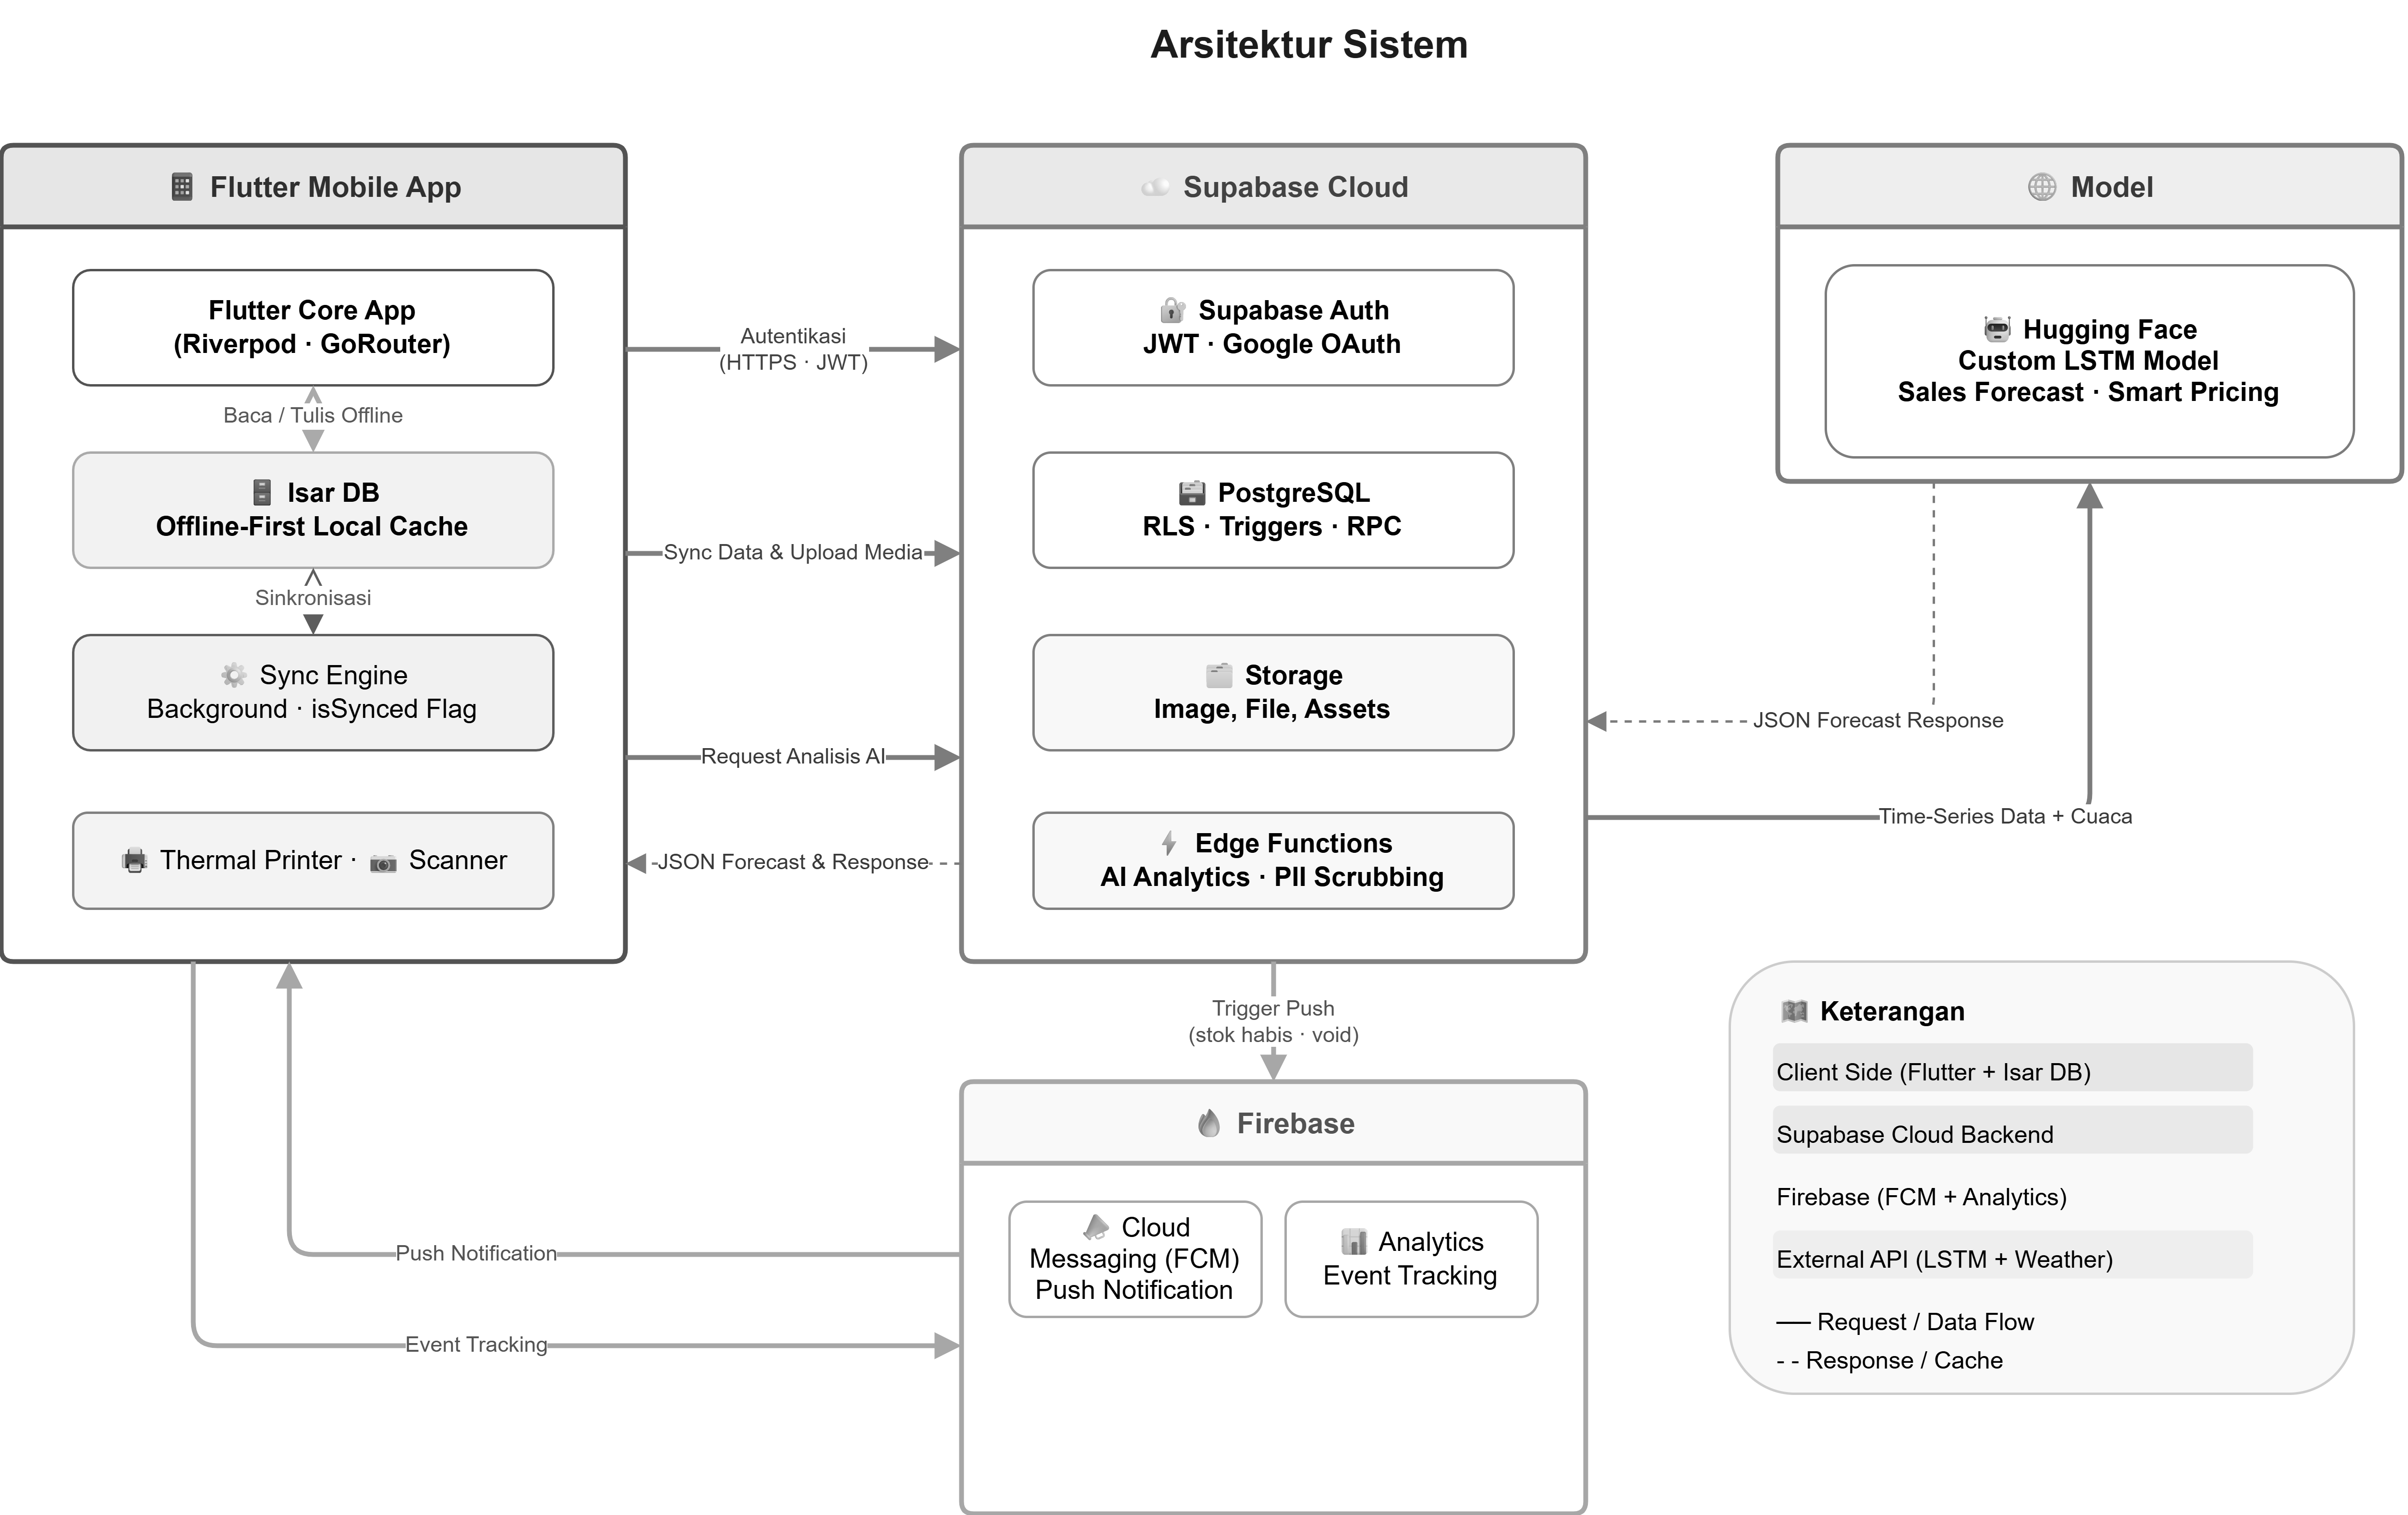
\includegraphics[width=0.75\textwidth]{arsitektur_sistem_bw.png}}{\fbox{POS System Architecture Diagram}}
  \caption{Architecture of the Offline-First Mobile POS System Integrated with LSTM Forecasting Services}
  \label{fig:alur_penelitian}
\end{figure}

\subsection{Offline-First POS System Architecture}
The system architecture was designed to guarantee uninterrupted cashier transactions without requiring persistent network connectivity. The platform consists of four primary components (Figure \ref{fig:alur_penelitian}):
\begin{itemize}
  \item Mobile Client Application: Built with Flutter (Dart programming language) following the Riverpod reactive state management architecture. Local persistence is managed by Isar Database, which stores product catalogs, categories, and receipts instantaneously. A background Sync Engine periodically monitors network connectivity; upon detecting an active internet connection, it dispatches unsynchronized local transaction records marked with \texttt{is\_synced = false} to the cloud database.
  \item Cloud Infrastructure (Supabase): Utilizes managed Supabase PostgreSQL as a centralized relational database equipped with Row Level Security (RLS) policies and a stored procedure (\textit{Remote Procedure Call}/RPC) named \texttt{create\_transaction\_v4} to execute atomic transaction records and inventory deductions.
  \item Telemetry and Messaging Services (Firebase): Employs Firebase Cloud Messaging (FCM) for broadcast announcements and low-stock push alerts, and Firebase Analytics for in-app operational telemetry.
  \item Predictive Inference Service (Hugging Face): The trained LSTM model is served via a Flask REST API on Hugging Face Spaces. The mobile client transmits aggregated historical revenue sequences via HTTPS and receives multi-step forecasting projections in structured JSON format.
\end{itemize}

\subsection{Dataset and Data Preprocessing}
The empirical dataset comprises authentic transactional records collected from the EatsTEDI SV UGM canteen between October 26, 2024, and September 4, 2025. Preprocessing was conducted through the following stages:
\begin{itemize}
  \item Active Day Filtering: Retained only operational business days with positive gross revenue ($\text{revenue} > 0$), resulting in 313 active sales days. Academic holiday closures and non-trading weekends were pruned to establish a continuous operational sequence.
  \item Target Log-Return Transformation: To mitigate non-stationarity and stabilize wide revenue variance, the target series was converted into daily log-returns ($r_t$):
  \begin{equation}
    r_t = \ln\left(\frac{Y_t + 1}{Y_{t-1} + 1}\right)
    \label{eq:log_return}
  \end{equation}
  where $Y_t$ represents the nominal gross sales revenue on active day $t$. The $+1$ offset prevents undefined values during zero-revenue anomalies.
  \item Cyclical Temporal Features: Extracted day-of-week calendar cycles using sine and cosine trigonometric transformations:
  \begin{equation}
    \sin_{\text{dow}} = \sin\left(\frac{2\pi \cdot d}{7}\right), \quad \cos_{\text{dow}} = \cos\left(\frac{2\pi \cdot d}{7}\right)
    \label{eq:dow}
  \end{equation}
  where $d \in \{0, 1, \dots, 6\}$ designates the day index within the weekly cycle.
  \item Normalization and Sequence Construction: Continuous numerical features were scaled into $[0, 1]$ via Min-Max Scaling. Supervised learning samples were generated using a sliding window across 7 active trading days ($look\_back = 7$), resulting in an input tensor dimension of $7 \times 8$.
  \item Chronological Dataset Splitting: Data was partitioned chronologically (time-based split) into 70\% training set (212 sequences), 15\% validation set (45 sequences), and 15\% testing set (46 sequences).
\end{itemize}

\subsection{Long Short-Term Memory (LSTM) Model Architecture}
The LSTM recurrent neural network was employed to learn temporal sequential patterns from sales history \cite{hochreiter1997}. Within each LSTM cell at time step $t$, state transitions are governed by four gating mechanisms:
\begin{align}
  \mathbf{f}_t &= \sigma\left(\mathbf{W}_f \cdot [\mathbf{h}_{t-1}, \mathbf{x}_t] + \mathbf{b}_f\right) \label{eq:forget_gate} \\
  \mathbf{i}_t &= \sigma\left(\mathbf{W}_i \cdot [\mathbf{h}_{t-1}, \mathbf{x}_t] + \mathbf{b}_i\right) \label{eq:input_gate} \\
  \tilde{\mathbf{C}}_t &= \tanh\left(\mathbf{W}_C \cdot [\mathbf{h}_{t-1}, \mathbf{x}_t] + \mathbf{b}_C\right) \label{eq:candidate_cell} \\
  \mathbf{C}_t &= \mathbf{f}_t \odot \mathbf{C}_{t-1} + \mathbf{i}_t \odot \tilde{\mathbf{C}}_t \label{eq:cell_update} \\
  \mathbf{o}_t &= \sigma\left(\mathbf{W}_o \cdot [\mathbf{h}_{t-1}, \mathbf{x}_t] + \mathbf{b}_o\right) \label{eq:output_gate} \\
  \mathbf{h}_t &= \mathbf{o}_t \odot \tanh(\mathbf{C}_t) \label{eq:hidden_state}
\end{align}
where $\mathbf{f}_t, \mathbf{i}_t, \mathbf{o}_t$ denote the forget gate, input gate, and output gate vectors, respectively; $\mathbf{C}_t$ represents the internal cell state; $\mathbf{h}_t$ denotes the hidden state; $\sigma(\cdot)$ is the logistic sigmoid activation; and $\odot$ represents element-wise multiplication (Hadamard product).

The layer configuration of the Hybrid LSTM model is summarized in Algorithm \ref{alg:lstm_model}, and the training hyperparameters are listed in Table \ref{tab:param_pelatihan}.

\begin{algorithm}[htbp]
\caption{Construction of Hybrid Residual LSTM Model Using TensorFlow/Keras}
\label{alg:lstm_model}
\fontsize{8.5pt}{10.5pt}\selectfont
\begin{algorithmic}[1]
\Require Input sequences $\mathbf{X}_t \in \mathbb{R}^{7 \times 8}$ ($look\_back = 7$, $n\_features = 8$).
\Ensure Predicted log-return of daily sales revenue $\hat{r}_t \in \mathbb{R}$.
\State $\text{model} \gets \text{Sequential}()$
\State $\text{model}.\text{add}(\text{LSTM}(\text{units}=24, \text{input\_shape}=(7, 8), \text{return\_sequences}=\text{False}))$
\State $\text{model}.\text{add}(\text{Dropout}(\text{rate}=0.1))$
\State $\text{model}.\text{add}(\text{Dense}(\text{units}=16, \text{activation}=\text{'relu'}))$
\State $\text{model}.\text{add}(\text{Dense}(\text{units}=1, \text{activation}=\text{'linear'}))$
\State $\text{model}.\text{compile}(\text{optimizer}=\text{Adam}(\text{lr}=5 \times 10^{-4}), \text{loss}=\text{'mse'}, \text{metrics}=[\text{'mae'}])$
\State \Return $\text{model}$
\end{algorithmic}
\end{algorithm}

\begin{table}[htbp]
  \centering
  \caption{Training Hyperparameter Specifications for the LSTM Model}
  \label{tab:param_pelatihan}
  \fontsize{8.5pt}{11pt}\selectfont
  \begin{tabular}{ll}
    \toprule
    \textbf{Hyperparameter} & \textbf{Value / Specification} \\
    \midrule
    Input Tensor Shape & $7 \times 8$ ($LOOK\_BACK = 7$ active days, 8 features) \\
    LSTM Hidden Layer & 1 layer, 24 LSTM cell units \\
    Dropout Rate & 0.1 \\
    Fully Connected Layer & Dense 16 units (ReLU activation) \\
    Output Layer & Dense 1 linear unit (log-return prediction) \\
    Total Trainable Parameters & 3,585 parameters \\
    Optimization Algorithm & Adam ($\text{learning rate} = 5 \times 10^{-4}$) \\
    Loss Function & Mean Squared Error (MSE) \\
    Batch Size & 16 \\
    Maximum Epochs & 200 (Early Stopping \textit{patience}=20 \& ReduceLROnPlateau) \\
    \bottomrule
  \end{tabular}
\end{table}

\subsection{Nominal Reconstruction and Multi-Step Projection}
The predicted log-return $\hat{r}_t$ was mapped back into nominal currency scale (IDR, $\hat{Y}_t$) via inverse exponential reconstruction:
\begin{equation}
  \hat{Y}_t = \exp\left(\ln(Y_{t-1} + 1) + \hat{r}_t\right) - 1
  \label{eq:rekonstruksi}
\end{equation}

For recursive multi-step forecasting extending up to 7 active business days ahead, three safety guards were enforced:
\begin{itemize}
  \item Clipping: Bound forecasted log-returns within the 10th and 90th empirical percentiles of the training distribution to prevent extreme deviations.
  \item Damping: Scaled projected variations by an exponential decay factor $\phi^{h-1}$ ($\phi = 0.7$) as the step horizon $h$ increases.
  \item Safety Rail: Clamped projected nominal sales revenue to never exceed the historical upper bound (revenue ceiling).
\end{itemize}

\subsection{Evaluation Metrics and Feasibility Benchmark}
Forecasting accuracy was examined under a one-step-ahead protocol utilizing three complementary evaluation metrics \cite{hyndman2006}:
\begin{align}
  \text{MAE} &= \frac{1}{N} \sum_{t=1}^N \left| Y_t - \hat{Y}_t \right| \label{eq:mae} \\
  \text{RMSE} &= \sqrt{\frac{1}{N} \sum_{t=1}^N \left( Y_t - \hat{Y}_t \right)^2} \label{eq:rmse} \\
  \text{sMAPE} &= \frac{100\%}{N} \sum_{t=1}^N \frac{\left| Y_t - \hat{Y}_t \right|}{\left( \left| Y_t \right| + \left| \hat{Y}_t \right| \right) / 2} \label{eq:smape}
\end{align}
where $Y_t$ denotes actual gross revenue, $\hat{Y}_t$ is the forecasted revenue, and $N$ represents the test sample size ($N=46$). Symmetric MAPE (sMAPE) serves as the primary benchmark because it provides bounded, scale-free percentage errors without diverging when encountering small sales values. The practical operational threshold was set at $\text{sMAPE} < 20\%$.

% =========================================================================
% Section 3: Results and Discussion
% =========================================================================
\section{Results and Discussion}

\subsection{Evaluation of LSTM Forecasting Model Against Practical Threshold}
Model performance on the test dataset (46 active days) was assessed across two rigorous evaluation scenarios. The first scenario benchmarked the one-step-ahead forecasting accuracy of the Hybrid LSTM model. The empirical evaluation metrics are summarized in Table \ref{tab:skenario1}.

\begin{table}[htbp]
  \centering
  \caption{Hybrid LSTM Model Performance on Test Dataset (One-Step-Ahead)}
  \label{tab:skenario1}
  \fontsize{8.5pt}{11pt}\selectfont
  \begin{tabular}{lccc}
    \toprule
    \textbf{Model / Architecture} & \textbf{MAE (IDR)} & \textbf{RMSE (IDR)} & \textbf{sMAPE (\%)} \\
    \midrule
    Hybrid LSTM (10-Seed Average) & 667,718 & 897,563 & 38.06\% \\
    \textbf{Practical Feasibility Threshold} & -- & -- & $\mathbf{< 20.00\%}$ \\
    \bottomrule
  \end{tabular}
\end{table}

As detailed in Table \ref{tab:skenario1}, the Hybrid LSTM model yielded an average MAE of IDR 667,718.00, RMSE of IDR 897,563.00, and sMAPE of 38.06\%. The sMAPE metric substantially exceeded the pre-established 20\% operational feasibility benchmark. The visual comparison between actual revenue and model forecasts is illustrated in Figure \ref{fig:prediksi_aktual}.

\begin{figure}[htbp]
  \centering
  \IfFileExists{Gambar/prediksi_vs_aktual.png}{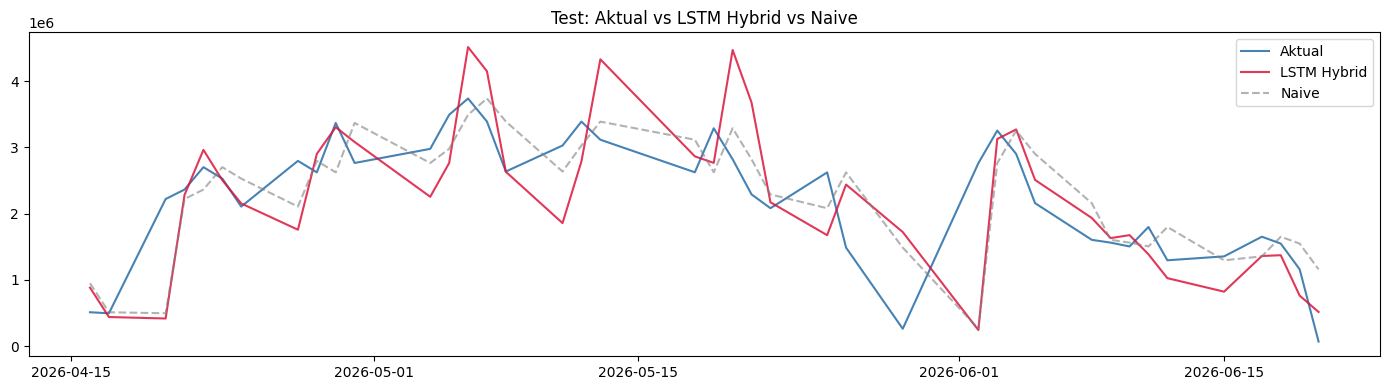
\includegraphics[width=0.75\textwidth]{prediksi_vs_aktual.png}}{\fbox{Actual vs Forecasted Revenue Plot}}
  \caption{Time Series Comparison of Actual Canteen Revenue Against Hybrid LSTM Model Forecasts}
  \label{fig:prediksi_aktual}
\end{figure}

The trajectory in Figure \ref{fig:prediksi_aktual} highlights that the LSTM model exhibited pronounced over-smoothing. While the model successfully approximated medium-term central revenue tendencies, it was unable to capture sudden, high-magnitude sales peaks induced by campus events and irregular academic schedules.

\subsection{Model Stability Testing via Multi-Seed Evaluation}
The second evaluation scenario tested model stability against random weight initialization variations. The training pipeline was executed 10 times under identical parameters using distinct random seeds ($seed \in \{0, 1, \dots, 9\}$). Descriptive performance statistics across the 10 runs are provided in Table \ref{tab:multiseed}.

\begin{table}[htbp]
  \centering
  \caption{Hybrid LSTM Performance Across Multi-Seed Stability Testing (10 Runs)}
  \label{tab:multiseed}
  \fontsize{8.5pt}{11pt}\selectfont
  \begin{tabular}{lccc}
    \toprule
    \textbf{Evaluation Metric} & \textbf{Mean} & \textbf{Std. Deviation ($\pm$)} & \textbf{Range (Min -- Max)} \\
    \midrule
    MAE (IDR)   & 667,718 & 145,024 & 495,527 -- 1,048,967 \\
    RMSE (IDR)  & 897,563 & 165,804 & 703,721 -- 1,320,587 \\
    sMAPE (\%)  & 38.06\% & 3.96\%  & 29.16\% -- 44.63\%   \\
    \bottomrule
  \end{tabular}
\end{table}

The empirical results in Table \ref{tab:multiseed} reveal considerable variance across seeds, exhibiting a standard deviation of IDR 145,024.00 in MAE and 3.96\% in sMAPE. The worst-performing initialization (MAE IDR 1,048,967.00) recorded an error more than double that of the best initialization (MAE IDR 495,527.00). Crucially, none of the 10 seeds reached the target sMAPE threshold of $< 20\%$ (the top-performing run achieved 29.16\% on Seed 7). The distribution of MAE values across runs is depicted as a boxplot in Figure \ref{fig:boxplot}.

\begin{figure}[htbp]
  \centering
  \IfFileExists{Gambar/boxplot_multiseed.png}{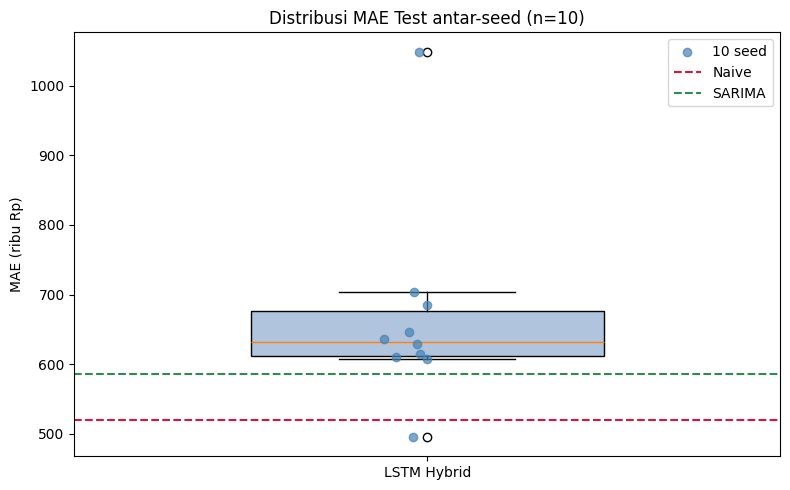
\includegraphics[width=0.48\textwidth]{boxplot_multiseed.png}}{\fbox{Multi-Seed MAE Boxplot}}
  \caption{MAE Error Distribution of Hybrid LSTM Across Multi-Seed Stability Runs (10 Iterations)}
  \label{fig:boxplot}
\end{figure}

This dispersion underscores that training neural networks on modest sequential datasets (212 training samples) is inherently prone to initialization instability (\textit{seed variance}). Consequently, reporting single-run performance for deep forecasting architectures on small datasets introduces significant reporting bias. A concise synthesis of both evaluation scenarios is presented in Table \ref{tab:rekap_skenario}.

\begin{table}[htbp]
  \centering
  \caption{Summary of Empirical Evaluation Scenarios for the Forecasting Model}
  \label{tab:rekap_skenario}
  \fontsize{8.5pt}{10.5pt}\selectfont
  \begin{tabularx}{\textwidth}{cp{4.2cm}cp{6.2cm}}
    \toprule
    \textbf{Scenario} & \textbf{Evaluation Objective} & \textbf{Threshold Met?} & \textbf{Key Empirical Finding} \\
    \midrule
    1 & Measure one-step-ahead accuracy against benchmark ($\text{sMAPE} < 20\%$) & No & Mean MAE IDR 667,718.00 and sMAPE 38.06\%, exceeding operational threshold. \\
    \midrule
    2 & Assess training stability across 10 randomized seeds & No & Wide MAE spread (IDR 495,527--1,048,967) with standard deviation IDR 145,024; 0 of 10 seeds satisfied sMAPE $< 20\%$. \\
    \bottomrule
  \end{tabularx}
\end{table}

\subsection{Mobile Point of Sale Interface Implementation}
The mobile POS application was deployed to Android mobile hardware featuring a modern, intuitive user interface. The system delivers complete cashier transaction workflows, catalog management, inventory adjustments, daily revenue dashboards, and a specialized Smart Analytics screen presenting 7-day predictive projections generated by the LSTM inference microservice (Figure \ref{fig:ui_smart_analytics}).

\begin{figure}[htbp]
  \centering
  \IfFileExists{Gambar/smart_analytics.png}{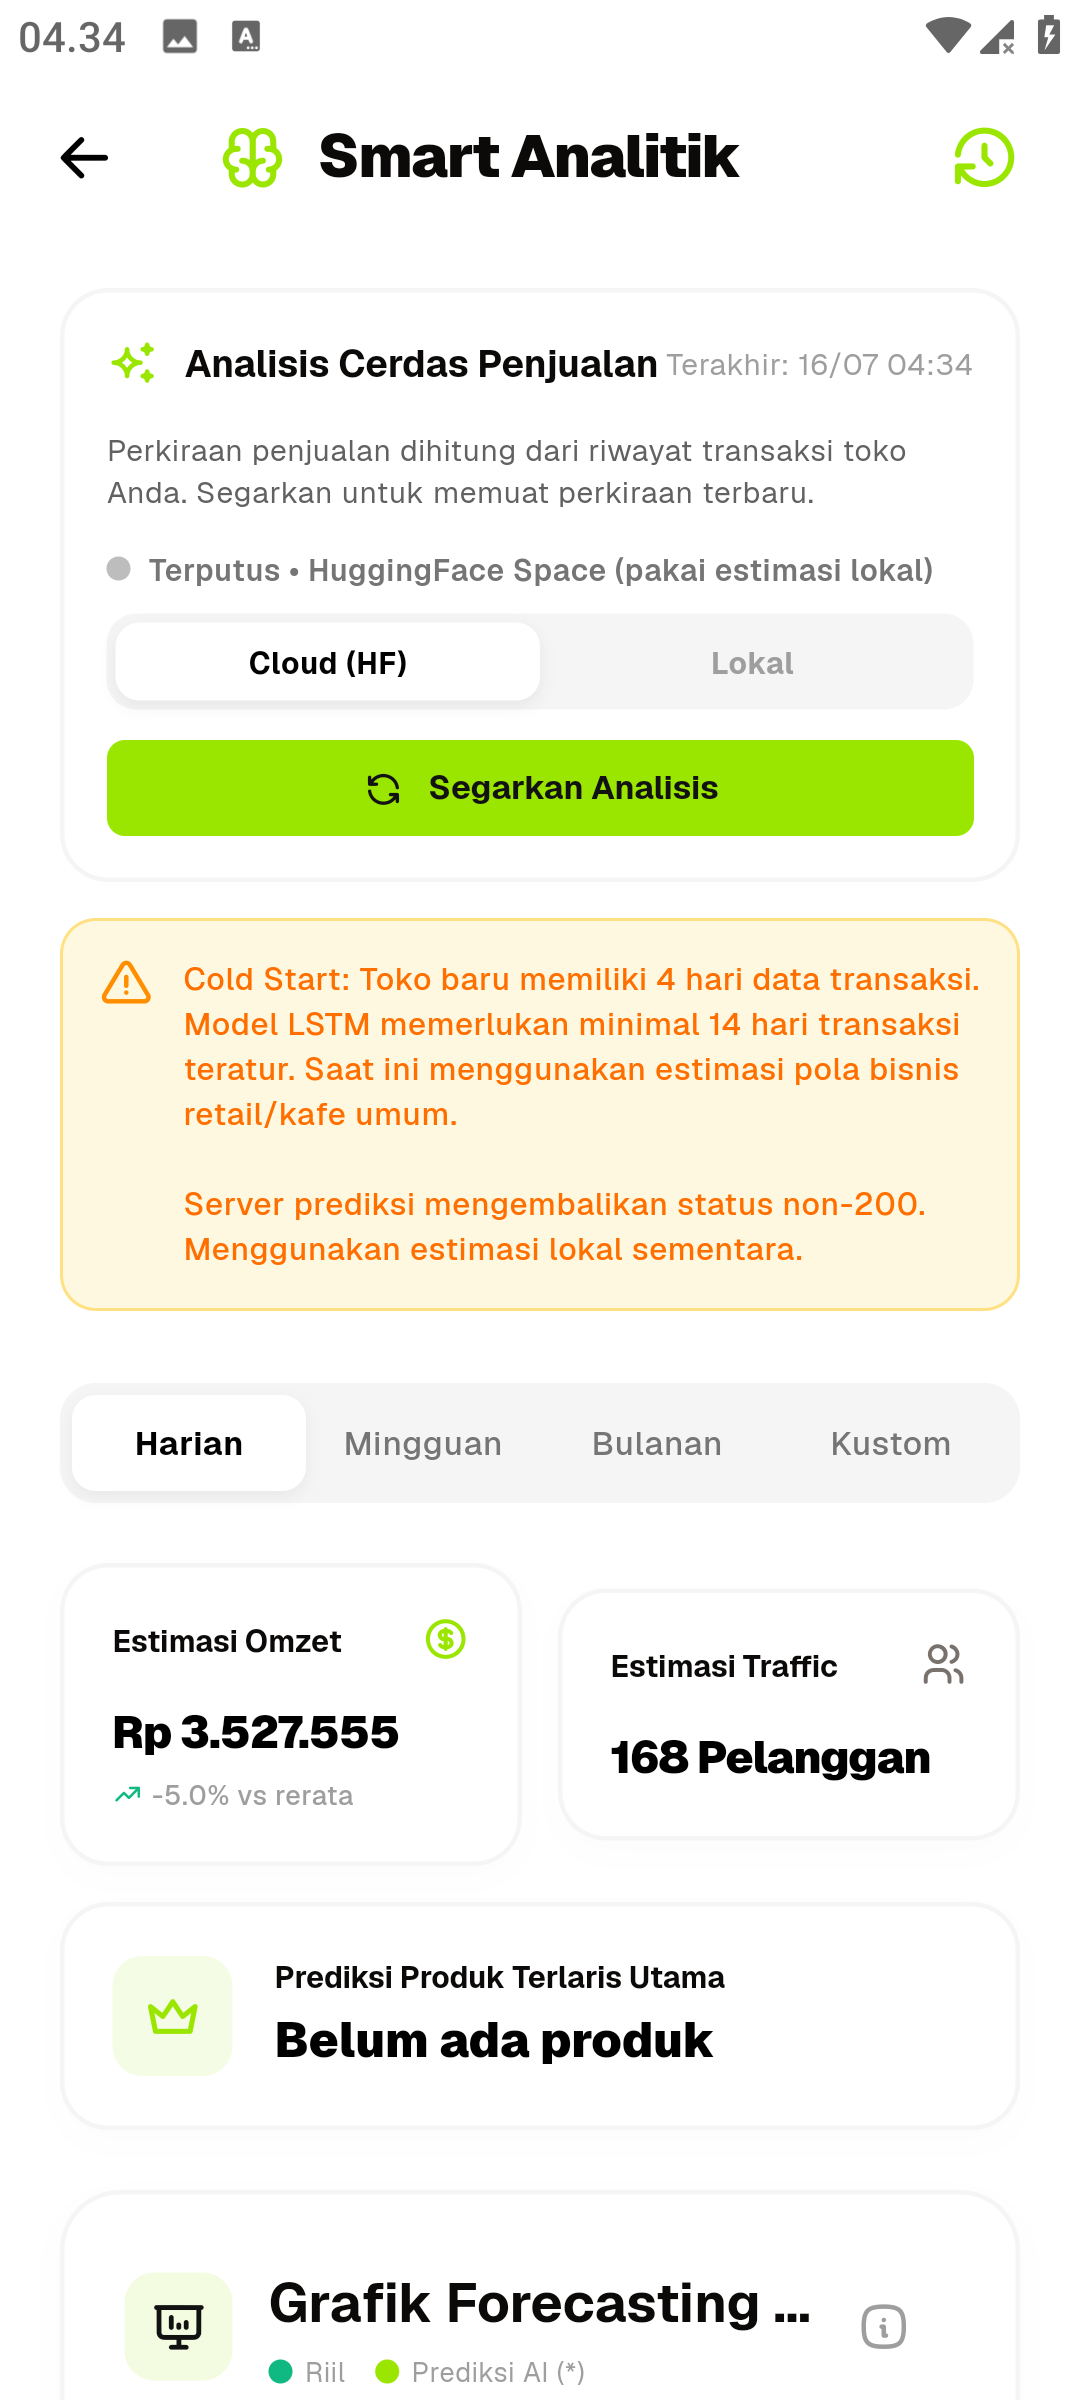
\includegraphics[width=0.45\textwidth]{smart_analytics.png}}{\fbox{POS Smart Analytics Interface}}
  \caption{User Interface of the Smart Analytics Module in the Mobile POS Application}
  \label{fig:ui_smart_analytics}
\end{figure}

The Smart Analytics module displays projected gross sales, multi-horizon trend charts with ceiling limits (safety rails), and cold-start detection banners that advise store operators when sales history has not yet reached the required 30-day warm-up baseline.

\subsection{Functional System Testing (Black Box Testing)}
Comprehensive black-box verification was executed across 12 core operational use cases covering both Owner and Cashier roles \cite{pressman2020, myers2011}. Every test case completed successfully with a 100\% PASS outcome (Table \ref{tab:blackbox}).

\begin{table}[htbp]
  \centering
  \caption{Black Box Test Outcomes Across Core Mobile POS Features}
  \label{tab:blackbox}
  \fontsize{8pt}{10pt}\selectfont
  \begin{tabularx}{\textwidth}{clXXc}
    \toprule
    \textbf{No} & \textbf{Feature / Test Case} & \textbf{Testing Action} & \textbf{Expected Result} & \textbf{Status} \\
    \midrule
    1 & Merchant Registration & Enter merchant profile \& store credentials & Account registered on cloud PostgreSQL & PASS \\
    2 & User Authentication   & Submit valid credentials                    & Dashboard access matched to user role & PASS \\
    3 & Checkout Transaction  & Select items \& confirm payment             & Local commit \& immediate stock deduction & PASS \\
    4 & Product Management    & Create, update, and delete menu items       & Catalog updated instantly in local DB & PASS \\
    5 & Category Organization & Organize menu category taxonomies          & Categories saved and displayed at register & PASS \\
    6 & Inventory Stock Audit & Review stock adjustment history log         & Accurate records of additions/deductions & PASS \\
    7 & Sales Dashboard       & Review daily turnover summaries             & Valid aggregation \& sales charts & PASS \\
    8 & Smart Analytics       & Request 7-day sales projections             & Projections displayed with bounds & PASS \\
    9 & Staff Notifications   & Dispatch broadcast message to staff         & FCM notification received on cashier app & PASS \\
    10& Data Synchronization  & Restore internet connectivity               & Queued transactions synced to cloud & PASS \\
    11& Staff Management      & Configure cashier accounts \& permissions   & Cashier role verified and updated & PASS \\
    12& Store Profile         & Update business name, address, and logo     & Profile propagated across all modules & PASS \\
    \bottomrule
  \end{tabularx}
\end{table}

\subsection{Evaluation of Offline-First Synchronization Mechanics}
In-depth testing of the offline-first architecture was conducted to ensure data integrity during offline-to-online transitions. Results are presented in Table \ref{tab:sinkronisasi}.

\begin{table}[htbp]
  \centering
  \caption{Validation Results of Offline-First Synchronization (Isar DB to Supabase)}
  \label{tab:sinkronisasi}
  \fontsize{8pt}{10.5pt}\selectfont
  \begin{tabularx}{\textwidth}{cp{4.5cm}Xc}
    \toprule
    \textbf{No} & \textbf{Test Scenario} & \textbf{Observed System Behavior} & \textbf{Status} \\
    \midrule
    1 & Checkout during offline state & Receipt saved in local Isar DB with \texttt{is\_synced = false}; inventory reduced locally. & PASS \\
    2 & View sales history offline    & Instant retrieval of local sales without network latency or UI blocking. & PASS \\
    3 & Reconnection to internet      & Sync Engine detects online status and uploads queued receipts via Supabase RPC. & PASS \\
    4 & Verify cloud data consistency & Transactions committed to Supabase without duplicates; local flag updated to \texttt{is\_synced = true}. & PASS \\
    \bottomrule
  \end{tabularx}
\end{table}

These findings demonstrate that embedding Isar DB provides near-instant cashier responsiveness while preserving total transactional integrity during network outages.

\subsection{Code Logic Path Testing (White Box Testing)}
White-box unit testing was conducted to verify critical conditional branches in the Python forecasting API service (Table \ref{tab:whitebox}).

\begin{table}[htbp]
  \centering
  \caption{White Box Test Verification of Critical Forecasting API Functions}
  \label{tab:whitebox}
  \fontsize{8pt}{10pt}\selectfont
  \begin{tabularx}{\textwidth}{clXXc}
    \toprule
    \textbf{No} & \textbf{Function / Target Path} & \textbf{Input Test Condition} & \textbf{Expected Execution Outcome} & \textbf{Status} \\
    \midrule
    1 & \texttt{by\_dow} (Seasonal-Naive) & Historical day-of-week data $\ge k$ & Computes mean across recent $k$ matching days & PASS \\
    2 & \texttt{by\_dow} (Partial Branch)  & Historical day-of-week data $< k$   & Computes mean across all available matching days & PASS \\
    3 & \texttt{by\_dow} (Fallback Path)   & Day-of-week completely missing      & Falls back to mean of last 10 active days & PASS \\
    4 & \texttt{smape} (Zero Denominator) & Actual and forecast values are zero & Denominator defaulted to 1; zero-division avoided & PASS \\
    5 & \texttt{forecast} (Clipping Guard)& Log-return exceeds percentile bound & Value clipped at empirical upper percentile & PASS \\
    6 & \texttt{forecast} (Damping Decay) & Forecast step $h > 1$               & Variance decayed by multiplicative factor $\phi^{h-1}$ & PASS \\
    7 & \texttt{forecast} (Safety Rail)   & Forecast exceeds historical max     & Nominal forecast clamped to historical ceiling & PASS \\
    \bottomrule
  \end{tabularx}
\end{table}

The white-box verification confirmed that all edge case exception routines and safety clamping logic functioned without runtime errors.

\subsection{Discussion and Findings Positioning}
Empirical findings demonstrate that the forecasting shortfall ($\text{sMAPE} = 38.06\%$) stems directly from the limited volume of historical training records (313 active days, 212 training sequences) paired with the sharp demand volatility characteristic of campus cafeteria environments. This aligns with findings from Makridakis et al. during the M5 Competition, where deep neural networks provided minimal competitive advantage over simpler statistical heuristics on brief time series lacking multi-year cyclical repetitions \cite{makridakis2022}. Furthermore, eliminating non-trading academic holidays ($\text{revenue} = 0$) created irregular calendar gaps between active business days, challenging the continuous time-step assumptions of recurrent neural architectures \cite{box2015}.

Nonetheless, this research contributes key engineering and methodological insights to applied predictive software development:
\begin{itemize}
  \item Multi-Seed Evaluation Transparency: Discloses neural network initialization variance through rigorous reporting of standard deviations and error bounds.
  \item Validity of sMAPE Metric: Prevents exploding percentage error artifacts encountered by standard MAPE when analyzing small-enterprise sales with near-zero baselines.
  \item Resilient Offline-First Architecture: Demonstrates the practical feasibility of pairing local Isar DB persistence with Supabase PostgreSQL to achieve zero cashier downtime regardless of connectivity status.
\end{itemize}

\FloatBarrier
% =========================================================================
% Section 4: Conclusion
% =========================================================================
\section{Conclusion and Future Work}

\subsection{Conclusion}
This research successfully engineered an offline-first mobile Point of Sale application utilizing Flutter, Isar Database, Supabase PostgreSQL, and a containerized LSTM forecasting REST microservice hosted on Hugging Face Spaces. Black-box functional validation across 12 primary use cases, offline synchronization verification, and white-box unit tests all achieved a 100\% PASS rate, confirming the system's ability to ensure zero downtime and near-instant checkout operations for MSMEs without continuous network connectivity. Regarding predictive modeling, empirical evaluation of the Hybrid LSTM model on 313 active days yielded an average MAE of IDR 667,718.00, RMSE of IDR 897,563.00, and sMAPE of 38.06\%, exceeding the practical feasibility threshold ($\text{sMAPE} < 20\%$). Multi-seed stability testing demonstrated substantial variance across runs (MAE IDR 495,527.00--1,048,967.00; sMAPE 29.16\%--44.63\%), indicating that deep recurrent architectures remain highly sensitive to weight initialization and require larger datasets to achieve stable convergence in micro-retail settings.

\subsection{Future Work}
Future research should expand data collection horizons across three to five operational years to enable deep sequence models to capture multi-year seasonal cycles effectively. Incorporating elapsed calendar gap features between non-consecutive trading days could alleviate temporal distortions caused by academic breaks. Additionally, future initiatives may explore transfer learning or multi-tenant global architectures across comparable retail categories to mitigate cold-start limitations, as well as investigate hybrid combinations (e.g., SARIMA-LSTM) that unify linear seasonal modeling with non-linear adaptation. Finally, enabling cryptographic encryption on the local Isar Database is recommended to further strengthen device-level data protection.

% =========================================================================
% References (IEEE Style)
% =========================================================================
\section*{References}

\begingroup
\renewcommand{\section}[2]{}%
\begin{thebibliography}{99}
\fontsize{8pt}{9.8pt}\selectfont
\setlength{\itemsep}{0.5pt}
\setlength{\parskip}{0pt}

\bibitem{sipayung2020}
E. M. Sipayung, C. Fiarni, and Wawan, 2020, ``Evaluation of Point of Sale Application Usage Using Technology Acceptance Model in MSMEs,'' \textit{Jurnal Nasional Teknik Elektro dan Teknologi Informasi (JNTETI)}, vol. 9, no. 1, pp. 18--24, Universitas Gadjah Mada, doi: 10.22146/jnteti.v9i1.116, ISSN: 2301-4156, URL: \url{https://doi.org/10.22146/jnteti.v9i1.116}, Abstract: Evaluation of POS adoption among MSMEs utilizing the Technology Acceptance Model focusing on perceived ease of use and usefulness., Keywords: Point of Sale, Technology Acceptance Model, MSME, Perceived Usefulness, Perceived Ease of Use, Document Type: Journal Article, Language: Indonesian, Database/Indexing: SINTA / Google Scholar, Citation Key: \texttt{sipayung2020}.

\bibitem{siddik2020}
M. Siddik and S. Samsir, 2020, ``Design and Implementation of POS (Point of Sale) Information System for Cashiers Using Object-Oriented Programming Concepts,'' \textit{JOISIE (Journal of Information Systems and Informatics Engineering)}, vol. 4, no. 1, pp. 43--49, Universitas Buana Perjuangan Karawang, doi: 10.35145/joisie.v4i1.607, ISSN: 2541-5506, URL: \url{https://doi.org/10.35145/joisie.v4i1.607}, Abstract: Development of an object-oriented POS cashier system for transactional efficiency and stock auditing., Keywords: Cashier Information System, Point of Sale, OOP, Java, Transaction Management, Document Type: Journal Article, Language: Indonesian, Database/Indexing: SINTA / Garuda, Citation Key: \texttt{siddik2020}.

\bibitem{flutter2026}
Google LLC, 2026, ``Flutter Documentation: Offline-first Architecture and Local Persistence,'' \textit{Google Developers}, Google LLC, URL: \url{https://docs.flutter.dev/}, Abstract: Official documentation on state management, asynchronous synchronization, offline caching patterns, and cross-platform native rendering., Keywords: Flutter, Offline-first, Local persistence, State management, Cross-platform, Document Type: Online Documentation, Language: English, Database/Indexing: Google Developers, Citation Key: \texttt{flutter2026}.

\bibitem{hyndman2021}
R. J. Hyndman and G. Athanasopoulos, 2021, ``Forecasting: Principles and Practice,'' \textit{OTexts}, 3rd ed., OTexts, Melbourne, Australia, ISSN: 978-0987507136, URL: \url{https://otexts.com/fpp3/}, Abstract: Comprehensive textbook on foundational time-series forecasting principles, exponential smoothing, ARIMA modeling, and accuracy evaluation., Keywords: Time series forecasting, ARIMA, Exponential smoothing, Error evaluation, Seasonality, Document Type: Book, Language: English, Database/Indexing: OTexts, Citation Key: \texttt{hyndman2021}.

\bibitem{box2015}
G. E. P. Box, G. M. Jenkins, G. C. Reinsel, and G. M. Ljung, 2015, ``Time Series Analysis: Forecasting and Control,'' \textit{John Wiley \& Sons}, 5th ed., John Wiley \& Sons, Inc., Hoboken, NJ, USA, doi: 10.1002/9781118619193, ISSN: 978-1-118-67502-1, URL: \url{https://doi.org/10.1002/9781118619193}, Abstract: Seminal work establishing classical Box-Jenkins methodology, autoregressive integrated moving average modeling, and transfer function controls., Keywords: Box-Jenkins, ARIMA, Autoregressive models, Stochastic processes, Time series, Document Type: Book, Language: English, Database/Indexing: Wiley Online Library, Citation Key: \texttt{box2015}.

\bibitem{hyndman2006}
R. J. Hyndman and A. B. Koehler, 2006, ``Another Look at Measures of Forecast Accuracy,'' \textit{International Journal of Forecasting}, vol. 22, no. 4, pp. 679--688, Elsevier B.V., doi: 10.1016/j.ijforecast.2006.03.001, ISSN: 0169-2070, URL: \url{https://doi.org/10.1016/j.ijforecast.2006.03.001}, Abstract: Systematic review and comparison of forecast accuracy metrics introducing symmetric MAPE and Mean Absolute Scaled Error for zero-value series., Keywords: Forecast accuracy, sMAPE, MASE, Metric comparison, Time series evaluation, Document Type: Journal Article, Language: English, Database/Indexing: Scopus / ScienceDirect, Citation Key: \texttt{hyndman2006}.

\bibitem{moraes2024}
T. de Castro Moraes, X.-M. Yuan, and E. P. Chew, 2024, ``Hybrid Convolutional Long Short-Term Memory Models for Sales Forecasting in Retail,'' \textit{Journal of Forecasting}, vol. 43, no. 5, pp. 1278--1293, John Wiley \& Sons, Ltd., doi: 10.1002/for.3073, ISSN: 0277-6693, URL: \url{https://doi.org/10.1002/for.3073}, Abstract: Development of a hybrid CNN-LSTM framework to capture both local spatial promotions and temporal sequential dependencies in retail store sales., Keywords: CNN-LSTM, Retail sales forecasting, Hybrid deep learning, Demand prediction, Time series, Document Type: Journal Article, Language: English, Database/Indexing: Scopus / Web of Science, Citation Key: \texttt{moraes2024}.

\bibitem{mansur2025}
S. Mansur, K. Sattar, S. E. Hosseini, S. Pervez, I. Ahmad, K. Saleem, and A. Z. Elhendi, 2025, ``Sales Forecasting for Retail Stores Using Hybrid Neural Networks and Sales-Affecting Variables,'' \textit{PeerJ Computer Science}, vol. 11, p. e3058, PeerJ Inc., doi: 10.7717/peerj-cs.3058, ISSN: 2376-5992, URL: \url{https://doi.org/10.7717/peerj-cs.3058}, Abstract: Novel hybrid deep neural network incorporating exogenous sales-affecting variables for multi-horizon store demand forecasting., Keywords: Sales forecasting, Deep learning, Hybrid neural networks, Feature engineering, Retail analytics, Document Type: Journal Article, Language: English, Database/Indexing: Scopus / PubMed Central, Citation Key: \texttt{mansur2025}.

\bibitem{mitra2024}
M. Mitra, S. Roy, S. De, S. Bhattacharyya, J. Platos, and V. Snasel, 2024, ``Harnessing LSTM Neural Networks and Hyperparameter Optimization for Precise Sales Forecasting in Retail,'' in \textit{Proc. 10th Int. Conf. Adv. Intell. Syst. Inform. (AISI 2024)}, ser. Lecture Notes on Data Engineering and Communications Technologies, vol. 220, pp. 120--131, Springer Cham, doi: 10.1007/978-3-031-71619-5\_11, ISSN: 2367-4520, URL: \url{https://doi.org/10.1007/978-3-031-71619-5_11}, Abstract: Application of hyperparameter-tuned LSTM architectures demonstrating robust sequential error reduction on volatile commercial sales records., Keywords: LSTM, Hyperparameter optimization, Retail sales forecasting, Grid search, Deep learning, Document Type: Conference Paper, Language: English, Database/Indexing: SpringerLink / Scopus, Citation Key: \texttt{mitra2024}.

\bibitem{yadav2025}
P. Yadav and C. R. Barde, 2025, ``Retail Real-Time Sales Prediction System Using LSTM and XGBoost,'' \textit{International Journal of Advanced Research in Computer and Communication Engineering (IJARCCE)}, vol. 14, no. 4, pp. 1--9, Tejasswvi Aadharnshila, doi: 10.17148/IJARCCE.2025.14401, ISSN: 2278-1021, URL: \url{https://ijarcce.com/}, Abstract: Real-time point-of-sale sales forecasting pipeline comparing gradient boosted decision trees against recurrent neural networks., Keywords: Sales prediction, LSTM, XGBoost, Real-time forecasting, Point of sale, Document Type: Journal Article, Language: English, Database/Indexing: Google Scholar, Citation Key: \texttt{yadav2025}.

\bibitem{sembiring2025}
R. A. Sembiring and Y. Sary, 2025, ``Analysis and Implementation of Long Short-Term Memory (LSTM) for Inventory Demand in PT. Gunung Sari Indonesia,'' \textit{Jurnal Ilmiah Teknik Mesin, Elektro dan Komputer}, vol. 5, no. 1, pp. 112--124, Universitas Bina Darma, ISSN: 2809-8404, URL: \url{https://journal.binadarma.ac.id/}, Abstract: Implementation of LSTM networks for warehouse inventory demand forecasting to prevent stockouts based on historical demand patterns., Keywords: LSTM, Inventory forecasting, Time series, Inventory management, Deep learning, Document Type: Journal Article, Language: Indonesian, Database/Indexing: SINTA / Garuda, Citation Key: \texttt{sembiring2025}.

\bibitem{jannah2025}
U. M. Jannah, D. S. Hormansyah, and D. P. Hapsari, 2025, ``Analysis of Water Refill Sales Prediction Using LSTM and SARIMA Methods,'' \textit{Jurnal Teknologi Informasi dan Multimedia}, vol. 7, no. 2, pp. 88--97, Politeknik Negeri Malang, ISSN: 2684-9666, URL: \url{https://jurnal.polinema.ac.id/}, Abstract: Performance comparison of SARIMA statistical models and LSTM deep learning on daily sales transactions of gallon water refill enterprises., Keywords: LSTM, SARIMA, Sales prediction, Time series, Model comparison, Document Type: Journal Article, Language: Indonesian, Database/Indexing: SINTA / Garuda, Citation Key: \texttt{jannah2025}.

\bibitem{verdiyanto2025}
R. Verdiyanto, D. Hartanti, and E. Purwanto, 2025, ``Development of Point of Sales Application for Beverage Enterprise Daily Sales Prediction Using Random Forest Regression Algorithm,'' \textit{Infotek: Jurnal Informatika dan Teknologi}, vol. 8, no. 2, pp. 310--321, STMIK Lombok, doi: 10.29408/jit.v8i2.25681, ISSN: 2614-8773, URL: \url{https://doi.org/10.29408/jit.v8i2.25681}, Abstract: Development of a Point of Sale application featuring daily sales prediction integrated with Random Forest ensemble regression., Keywords: Point of Sale, Random Forest Regression, Daily prediction, Beverage MSME, Machine learning, Document Type: Journal Article, Language: Indonesian, Database/Indexing: SINTA / Garuda, Citation Key: \texttt{verdiyanto2025}.

\bibitem{hochreiter1997}
S. Hochreiter and J. Schmidhuber, 1997, ``Long Short-Term Memory,'' \textit{Neural Computation}, vol. 9, no. 8, pp. 1735--1780, MIT Press, doi: 10.1162/neco.1997.9.8.1735, ISSN: 0899-7667, URL: \url{https://doi.org/10.1162/neco.1997.9.8.1735}, Abstract: Seminal introduction of the Long Short-Term Memory recurrent neural network solving the vanishing and exploding gradient problems., Keywords: Long Short-Term Memory, Recurrent neural networks, Gradient descent, Sequential learning, Deep learning, Document Type: Journal Article, Language: English, Database/Indexing: Scopus / Web of Science, Citation Key: \texttt{hochreiter1997}.

\bibitem{goodfellow2016deep}
I. Goodfellow, Y. Bengio, and A. Courville, 2016, ``Deep Learning,'' \textit{MIT Press}, MIT Press, Cambridge, MA, USA, ISSN: 978-0262035613, URL: \url{https://www.deeplearningbook.org/}, Abstract: Comprehensive textbook covering mathematical foundations, deep feedforward architectures, regularization, and sequence modeling., Keywords: Deep learning, Neural networks, Optimization, Representation learning, Sequence modeling, Document Type: Book, Language: English, Database/Indexing: MIT Press, Citation Key: \texttt{goodfellow2016deep}.

\bibitem{makridakis2022}
S. Makridakis, E. Spiliotis, and V. Assimakopoulos, 2022, ``The M5 Competition: Background, Organization, and Implementation,'' \textit{International Journal of Forecasting}, vol. 38, no. 4, pp. 1325--1336, Elsevier B.V., doi: 10.1016/j.ijforecast.2021.07.007, ISSN: 0169-2070, URL: \url{https://doi.org/10.1016/j.ijforecast.2021.07.007}, Abstract: Overview of the global M5 forecasting competition evaluating machine learning and statistical methods on hierarchically aggregated retail data., Keywords: M5 Competition, Retail sales, Machine learning, Benchmark forecasting, Hierarchical time series, Document Type: Journal Article, Language: English, Database/Indexing: Scopus / ScienceDirect, Citation Key: \texttt{makridakis2022}.

\bibitem{pressman2020}
R. S. Pressman and B. R. Maxim, 2020, ``Software Engineering: A Practitioner's Approach,'' \textit{McGraw-Hill Education}, 9th ed., McGraw-Hill Education, New York, NY, USA, ISSN: 978-1259872976, Abstract: Foundational software engineering textbook detailing agile methodologies, design patterns, testing frameworks, and quality assurance., Keywords: Software engineering, Black box testing, System design, Quality assurance, Software metrics, Document Type: Book, Language: English, Database/Indexing: McGraw-Hill, Citation Key: \texttt{pressman2020}.

\bibitem{myers2011}
G. J. Myers, C. Sandler, and T. Badgett, 2011, ``The Art of Software Testing,'' \textit{John Wiley \& Sons}, 3rd ed., John Wiley \& Sons, Inc., Hoboken, NJ, USA, doi: 10.1002/9781119202486, ISSN: 978-1-118-03196-4, URL: \url{https://doi.org/10.1002/9781119202486}, Abstract: Authoritative guide on practical software verification, boundary value analysis, functional testing, and code inspection techniques., Keywords: Software testing, Black box testing, Equivalence partitioning, Test cases, Quality verification, Document Type: Book, Language: English, Database/Indexing: Wiley Online Library, Citation Key: \texttt{myers2011}.

\bibitem{iso2021}
ISO/IEC/IEEE 29119-4:2021, 2021, ``Software and Systems Engineering --- Software Testing --- Part 4: Test Techniques,'' \textit{International Organization for Standardization}, ISO/IEC/IEEE, Geneva, Switzerland, URL: \url{https://www.iso.org/standard/79016.html}, Abstract: International standard specifying rigorous test design techniques for black-box, white-box, and experience-based software verification., Keywords: ISO/IEC/IEEE 29119, Software testing standards, Test techniques, Verification, Quality control, Document Type: Standard, Language: English, Database/Indexing: ISO Standards, Citation Key: \texttt{iso2021}.
\end{thebibliography}
\endgroup

\end{document}
